\tocchapter{Softwarearen garapenerako prozesu bateratua}

\section{Eskakizunen bilketa}
Gure aplikazioak eduki behar dituen eskakizun funtzionalak zehazteko, hau da, aktoreen beharrak zerrendatzeko, balio du eskakizunen bilketak. Gure kasuan aktore bakarra izango dugu, \textbf{erabiltzailea} hain zuzen ere. Hauek dira bere eskakizunak:
\subsection{Azpitituluen inguruko eskakizunak}
\begin{itemize}
\item ASS eta SRT motako azpitituluak irekitzea eta gordetzea.
\item Azpititulu fitxategi berriak sortzeko aukera.
\item TXT fitxategietatik dialogoak inportatzea.
\item Fitxategiaren goiburukoen edizioa.
\item Lerro bakoitzaren eremuen gaineko edizioa: aktorea, estiloa, testua, denborak, etab. aldatzea.
\item Lerroen gaineko eragiketak: gehitu, kendu, \textit{shift}, \textit{split}, \textit{join}, bikoiztu, etab.
\item Sintaxia nabarmendua erosoago lan egiteko: ASS komandoen identifikazioa eta koloreztatzea.
\end{itemize}
\subsection{\textit{Typesetting}-aren inguruko eskakizunak}
\begin{itemize}
\item Estilo editorea estilo berriak sortzeko edo daudenak aldatzeko.
\item Estilo kudeatzailea, estiloak gorde ahal izateko edo \textit{script} batean txertatzeko.
\end{itemize}
\subsection{Tresna edo laguntzaileen inguruko eskakizunak}
\begin{itemize}
\item Itzulpenak egiteko laguntzailea.
\item Zuzentzaile ortografikoa.
\item Estiloak aplikatzeko laguntzailea.
\end{itemize}
\subsection{Bestelako eskakizunak}
\begin{itemize}
\item Lana periodikoki gordetzea modu automatikoan.
\item Dokumentu anitz irekita edukitzea aldi berean.
\item Undo/Redo aukerak.
\end{itemize}

\section{Analisia}
Nahiz eta programak zenbait formaturekin lan egin ahalko duen (ASS, SRT eta TXT), formatu \textit{natiboa} ASS izango da. Honen arrazoia zera da: ASS formatuak badauka SRT eta TXT formatuek eskaintzen duten guztia, baina alderantziz ez, hau da, ASS formatua askoz aurreratuagoa da. 

\begin{figure}[htp]
\begin{center}
%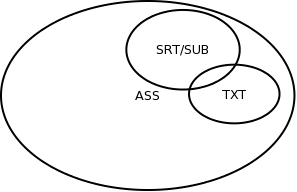
\includegraphics[width=\columnwidth, natwidth=555pt, natheight=402pt]{Pictures/Chapter4/Analisia/formatuak.png}
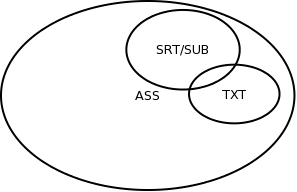
\includegraphics[scale=0.5]{Pictures/Chapter4/Analisia/formatuak.png}
\caption{Azpititulu formatuak}
\label{formatuak}
\end{center}
\end{figure}

\ref{formatuak}~Irudian ikusten denez, SRT eta TXT formatuak ASS formatuaren azpimultzoak direla esan daiteke. SRT formatuak dialogoak eta hauen hasiera eta bukaera denborak dauzka, eta TXT formatuak ordea, dialogoak eta hauen aktoreak bakarrik eskaintzen ditu.
\subsection{Domeinuaren eredua}
\ref{de}~Irudian ikusten denez, domeinuko osagaien izenak ingeleraz daude, honako arrazoiengatik: alde batetik, ASS formatuaren espezifikazioan izenak ingeleraz agertzen direlako\cite{gu:ass}, eta bestetik programa askea izango denez, norbaitek kodea irakurri edo hobetu nahi badu, askoz errazagoa izango da ingelera jakitea euskara ordez.
\begin{figure}[htp]
\begin{center}
%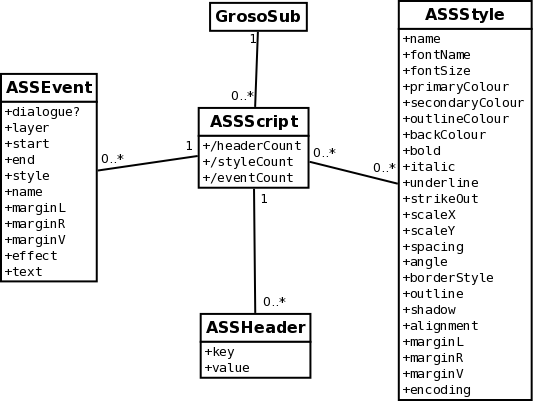
\includegraphics[width=\columnwidth, natwidth=555pt, natheight=402pt]{Pictures/Chapter4/Analisia/DE.png}
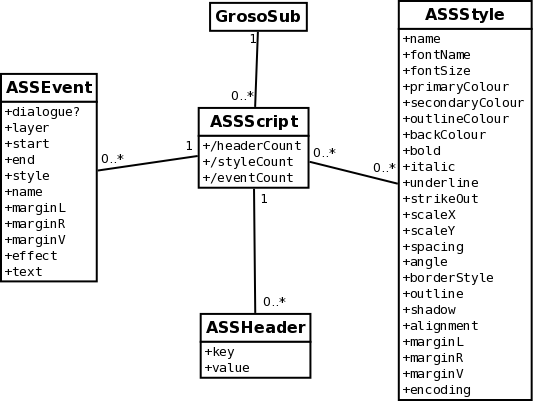
\includegraphics[scale=0.35]{Pictures/Chapter4/Analisia/DE.png}
\caption{Domeinuaren eredua}
\label{de}
\end{center}
\end{figure}

\subsection{Egoera diagrama}
Programaren izaera dela eta, egoera desberdinekin aurkituko gara. Definituko diren egoeratan zenbait erabilpen kasu gauzatu ahalko ditugu, batzutan beste egoera batzuetara pasaz. Honako diagraman ikus daitezke egoerak:

\begin{figure}[htp]
\begin{center}
%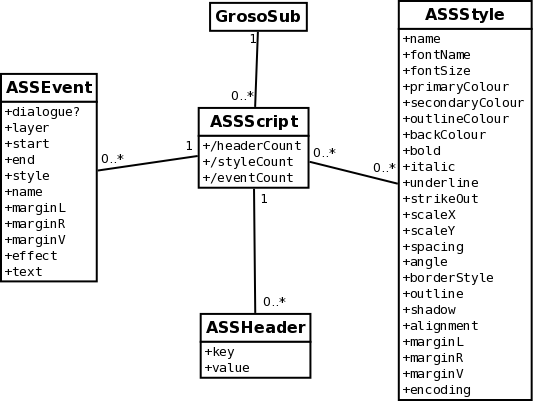
\includegraphics[width=\columnwidth, natwidth=555pt, natheight=402pt]{Pictures/Chapter4/Analisia/DE.png}
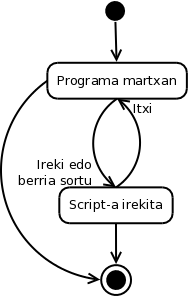
\includegraphics[scale=0.4]{Pictures/Chapter4/Analisia/ED.png}
\caption{Egoera diagrama}
\label{ed}
\end{center}
\end{figure}
\newpage
\subsection{Erabilpen kasuak}
\subsubsection{Egoera guztietan egin daitezkeenak}
\begin{figure}[htp]
\begin{center}
%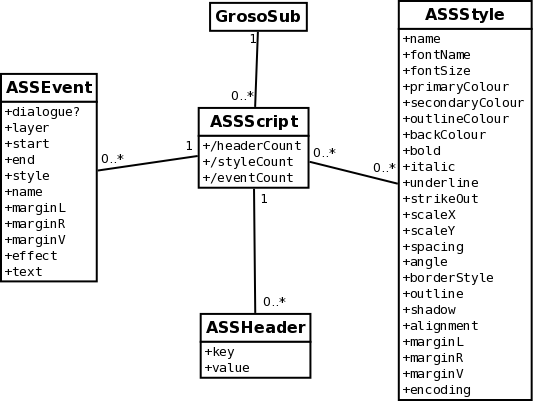
\includegraphics[width=\columnwidth, natwidth=555pt, natheight=402pt]{Pictures/Chapter4/Analisia/DE.png}
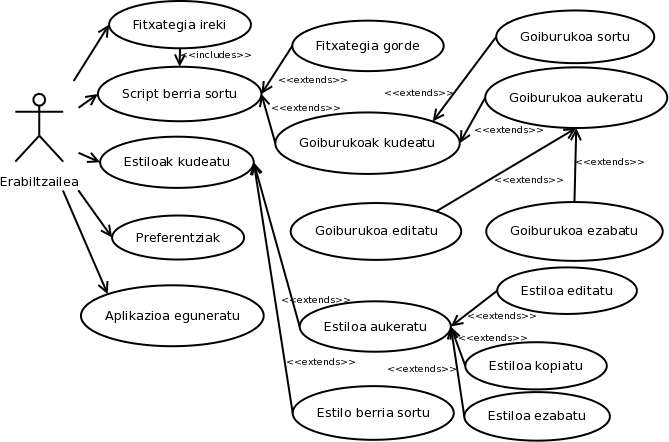
\includegraphics[scale=0.4]{Pictures/Chapter4/Analisia/EKE-Guztiak.png}
\caption{EKE - Egoera guztiak}
\label{eke-guztiak}
\end{center}
\end{figure}
\noindent\\
\textbf{ID:} G01.\\
\textbf{Erabilpen kasua:} Fitxategia ireki.\\
\textbf{Aktoreak:} Erabiltzailea.\\
\textbf{Deskribapena:} Fitxategi sisteman dagoen fitxategi bat kargatzen du.\\
\textbf{Aurrebaldintzak:} Fitxategia existitzen da.\\
\textbf{Postbaldintzak:} Fitxategia kargatuta geratzen da.\\
\textbf{Gertaera fluxu normala:}
\begin{enumerate}
	\item \textit{Erabiltzailea:} Fitxategi sistemako fitxategi bat aukeratzen du.
	\item \textit{Sistema:} Script berri bat sortzen du (\underline{includes: G02}).
	\item \textit{Sistema:} Sortu berri duen script-ean aukeratutako fitxategiko datuak kargatzen ditu.
	\item \textit{Sistema:} Erabiltzaileari erakusten dio lehio berri batean.
\end{enumerate}
\textbf{Gertaera fluxu alternatiboa:}
\begin{itemize}
	\item 3. urratsa: fitxategiaren formatua ez da zuzena.
		\begin{enumerate}
		\item \textit{Sistema:} Erabiltzaileari errorearen berri emango dio.
		\item \textit{Erabiltzailea:} Fitxategi berri bat aukeratuko du edo erabilpen kasutik aterako da.
		\end{enumerate}
\end{itemize}
\line(1,0){390}\\
\noindent\\
\textbf{ID:} G02.\\
\textbf{Erabilpen kasua:} Script berria sortu.\\
\textbf{Aktoreak:} Erabiltzailea.\\
\textbf{Deskribapena:} Script berri bat sortzen da defektuzko balioekin.\\
\textbf{Aurrebaldintzak:}\\
\textbf{Postbaldintzak:} Script-a sortzen da eta erabiltzaileari erakusten zaio.\\
\textbf{Gertaera fluxu normala:}
\begin{enumerate}
	\item \textit{Sistema:} Script berria sortzen du eta defektuzko informazioarekin osatzen du.
	\item \textit{Sistema:} Erabiltzaileari erakusten dio lehio berri batean.
\end{enumerate}
\line(1,0){390}\\
\noindent\\
\textbf{ID:} G03.\\
\textbf{Erabilpen kasua:} Fitxategia gorde.\\
\textbf{Aktoreak:} Erabiltzailea.\\
\textbf{Deskribapena:} Irekita dagoen script-a fitxategi batean gordetzen du aukeratutako formatuan.\\
\textbf{Aurrebaldintzak:} Script-a irekita dago.\\
\textbf{Postbaldintzak:} Script-a fitxategi sistemako fitxategi batean gordeta geratzen da.\\
\textbf{Gertaera fluxu normala:}
\begin{enumerate}
	\item \textit{Erabiltzailea:} Gordetzeko izena, lekua eta formatua aukeratuko ditu.
	\item \textit{Sistema:} Dagokion formatuan gordeko du irekita dagoen script-a.
\end{enumerate}
%\line(1,0){390}\\
\newpage
\noindent\\
\textbf{ID:} G04.\\
\textbf{Erabilpen kasua:} Goiburukoak kudeatu.\\
\textbf{Aktoreak:} Erabiltzailea.\\
\textbf{Deskribapena:} Irekita dagoen script-aren goiburukoak editatzen ditu.\\
\textbf{Aurrebaldintzak:} Script-a irekita dago.\\
\textbf{Postbaldintzak:} Goiburukoetan egindako aldaketak script-ean gordeta geratuko dira.\\
\textbf{Gertaera fluxu normala:}
\begin{enumerate}
	\item \textit{Sistema:} Script-ean dauden goiburuak zerrendatuko ditu.
	\item \textit{Erabiltzailea:} Goiburuko bat aukeratuko du editatzeko edo ezabatzeko, edo goiburuko berri bat sortuko du.
	\item \textit{Sistema:} Erabiltzaileak aukeratutako ekintza egingo du.
	\item \textit{Erabiltzailea:} Berriro egiteko edo irtetzeko aukera izango du.
	\item \textit{Sistema:} egin diren aldaketak script-ean gordeko ditu.
\end{enumerate}
\textbf{Gertaera fluxu alternatiboa:}
\begin{itemize}
	\item 4. urratsa: berriro egitea aukeratuko du erabiltzaileak:
		\begin{enumerate}
		\item \textit{Sistema:} Goiburukoen zerrenda eguneratuko du egin den azken aldaketa bertan isladatzeko.
		\item \textit{Erabiltzailea:} Beste goiburuko bat aukeratuko du editatzeko edo ezabatzeko, edo goiburuko berri bat sortuko du.
		\end{enumerate}
\end{itemize}
\line(1,0){390}\\
\noindent\\
\textbf{ID:} G05.\\
\textbf{Erabilpen kasua:} Goiburukoa sortu.\\
\textbf{Aktoreak:} Erabiltzailea.\\
\textbf{Deskribapena:} Irekita dagoen script-ean goiburuko berri bat sortzen du.\\
\textbf{Aurrebaldintzak:} Goiburukoen kudeatzailea martxan dago.\\
\textbf{Postbaldintzak:} Goiburuko berria goiburukoen zerrendan gordeko da.\\
\textbf{Gertaera fluxu normala:}
\begin{enumerate}
	\item \textit{Sistema:} Goiburuko berria sortzen du defektuzko balioekin eta goiburukoen zerrendan gordeko du.
\end{enumerate}
%\line(1,0){390}\\
\noindent\\
\textbf{ID:} G06.\\
\textbf{Erabilpen kasua:} Goiburukoa aukeratu.\\
\textbf{Aktoreak:} Erabiltzailea.\\
\textbf{Deskribapena:} Goiburuko bat aukeratzen du honekin zenbait eragiketa egin ahal izateko.\\
\textbf{Aurrebaldintzak:} Goiburukoen kudeatzailea martxan dago.\\
\textbf{Postbaldintzak:} Goiburuko bat aukeratuta geratzen da.\\
\textbf{Gertaera fluxu normala:}
\begin{enumerate}
	\item \textit{Erabiltzailea:} Goiburuko bat aukeratuko du goiburukoen zerrendatik.
	\item \textit{Sistema:} Erabiltzaileak aukeratutako goiburukoa markatuko du interfazean.
\end{enumerate}
\line(1,0){390}\\
\noindent\\
\textbf{ID:} G07.\\
\textbf{Erabilpen kasua:} Goiburukoa editatu.\\
\textbf{Aktoreak:} Erabiltzailea.\\
\textbf{Deskribapena:} Aukeratutako goiburukoaren balioa aldatzen du.\\
\textbf{Aurrebaldintzak:} Goiburuko bat aukeratuta dago.\\
\textbf{Postbaldintzak:} Aukeratutako goiburukoa aldatuta geratzen da script-ean.\\
\textbf{Gertaera fluxu normala:}
\begin{enumerate}
	\item \textit{Sistema:} Aukeratutako goiburukoaren balioa erakusten du.
	\item \textit{Erabiltzailea:} Balio berria sartzen du.
	\item \textit{Sistema:} Erabiltzaileak sartutako balioa goiburukoen zerrendan gordetzen du.
\end{enumerate}
\line(1,0){390}\\
\noindent\\
\textbf{ID:} G08.\\
\textbf{Erabilpen kasua:} Goiburukoa ezabatu.\\
\textbf{Aktoreak:} Erabiltzailea.\\
\textbf{Deskribapena:} Aukeratutako goiburukoa ezabatzen du script-etik.\\
\textbf{Aurrebaldintzak:} Goiburuko bat aukeratuta dago.\\
\textbf{Postbaldintzak:} Goiburukoa ezabatuko da script-etik.\\
\textbf{Gertaera fluxu normala:}
\begin{enumerate}
	\item \textit{Sistema:} Goiburukoa zerrendatik ezabatuko du.
\end{enumerate}
\line(1,0){390}\\
\noindent\\
\textbf{ID:} G09.\\
\textbf{Erabilpen kasua:} Estiloak kudeatu.\\
\textbf{Aktoreak:} Erabiltzailea.\\
\textbf{Deskribapena:} Estilo kudeatzailea agertuko da, script-ean eta biltegian dauden estiloak kudeatzeko.\\
\textbf{Aurrebaldintzak:} Script-a kargatuta dago.\\
\textbf{Postbaldintzak:} Estilo kudeatzailea kargatuko da.\\
\textbf{Gertaera fluxu normala:}
\begin{enumerate}
	\item \textit{Sistema:} Biltegian dauden estiloak eta script-ean daudenak zerrendatuko ditu.
	\item \textit{Sistema:} Estiloak kudeatzeko kontrolak kargatuko ditu.
\end{enumerate}
\line(1,0){390}\\
\noindent\\
\textbf{ID:} G10.\\
\textbf{Erabilpen kasua:} Estilo berria sortu.\\
\textbf{Aktoreak:} Erabiltzailea.\\
\textbf{Deskribapena:} Estilo berria sortuko eta editatuko du.\\
\textbf{Aurrebaldintzak:} Estilo kudeatzailean dago programa.\\
\textbf{Postbaldintzak:} Estiloa gordeta geratuko da.\\
\textbf{Gertaera fluxu normala:}
\begin{enumerate}
	\item \textit{Erabiltzailea:} Estiloa script-ean edo biltegian gordetzea aukeratuko du.
	\item \textit{Sistema:} Estilo berri bat sortuko du defektuzko aukerekin.
	\item \textit{Sistema:} Sortu berri duen estiloa editatzeko aukera emango dio erabiltzaileari (\underline{includes G12}).
	\item \textit{Sistema:} Estiloa gordeko du aukeratutako tokian.
\end{enumerate}
\line(1,0){390}\\
\noindent\\
\textbf{ID:} G11.\\
\textbf{Erabilpen kasua:} Estiloa aukeratu.\\
\textbf{Aktoreak:} Erabiltzailea.\\
\textbf{Deskribapena:} Biltegian edo script-ean dagoen estilo bat aukeratzen du ondoren eragiketaren bat egiteko.\\
\textbf{Aurrebaldintzak:} Estilo kudeatzailean dago programa.\\
\textbf{Postbaldintzak:} Estiloa aukeratuta geratzen da.\\
\textbf{Gertaera fluxu normala:}
\begin{enumerate}
	\item \textit{Erabiltzailea:} Biltegiko edo script-eko estilo zerrendan dagoen estilo bat aukeratzen du.
	\item \textit{Sistema:} Erabiltzaileak aukeratutako estiloa markatzen du interfazean eta dagozkion kontrolak aktibatzen ditu.
\end{enumerate}
\line(1,0){390}\\
\noindent\\
\textbf{ID:} G12.\\
\textbf{Erabilpen kasua:} Estiloa editatu.\\
\textbf{Aktoreak:} Erabiltzailea.\\
\textbf{Deskribapena:} Aukeratutako estiloaren eremuak editatzen ditu.\\
\textbf{Aurrebaldintzak:} Estilo bat aukeratuta dago.\\
\textbf{Postbaldintzak:} Estiloa gordetzen du dagokion lekuan aldaketa berriekin.\\
\textbf{Gertaera fluxu normala:}
\begin{enumerate}
	\item \textit{Sistema:} Aukeratutako estiloaren eremuak eta hauen balioak pantailaratzen ditu.
	\item \textit{Erabiltzailea:} Eremu bat aukeratzen du eta bere balioa aldatzen du.
	\item \textit{Erabiltzailea:} Beste eremu bat aukeratu (2. urratsa) edo irten daiteke.
	\item \textit{Sistema:} Estiloa gordetzen du.
\end{enumerate}
\line(1,0){390}\\
\noindent\\
\textbf{ID:} G13.\\
\textbf{Erabilpen kasua:} Estiloa kopiatu.\\
\textbf{Aktoreak:} Erabiltzailea.\\
\textbf{Deskribapena:} Estiloa kopiatzen du biltegitik script-era edo alderantziz.\\
\textbf{Aurrebaldintzak:} Estilo bat aukeratuta dago.\\
\textbf{Postbaldintzak:} Estiloa kopiatzen da.\\
\textbf{Gertaera fluxu normala:}
\begin{enumerate}
	\item \textit{Sistema:} Estiloa kopiatzen du leku batetik bestera.
	\item \textit{Sistema:} Estilo zerrenda eguneratzen du.
\end{enumerate}
\textbf{Gertaera fluxu alternatiboa:}
\begin{itemize}
	\item 1. urratsa: helburuan badago izen berdineko estiloa:
		\begin{enumerate}
		\item \textit{Sistema:} Izen berria emango dio estiloari, zenbaki bat parentesi tartean txertatuz izenaren amaieran.
		\end{enumerate}
\end{itemize}
\line(1,0){390}\\
\noindent\\
\textbf{ID:} G14.\\
\textbf{Erabilpen kasua:} Estiloa ezabatu.\\
\textbf{Aktoreak:} Erabiltzailea.\\
\textbf{Deskribapena:} Aukeratutako estiloa dagokion tokitik ezabatzen du.\\
\textbf{Aurrebaldintzak:} Estilo bat aukeratuta dago.\\
\textbf{Postbaldintzak:} Estiloa ezabatzen da.\\
\textbf{Gertaera fluxu normala:}
\begin{enumerate}
	\item \textit{Sistema:} Estiloa ezabatuko du dagokion lekutik.
\end{enumerate}
\line(1,0){390}\\
\noindent\\
\textbf{ID:} G15.\\
\textbf{Erabilpen kasua:} Preferentziak.\\
\textbf{Aktoreak:} Erabiltzailea.\\
\textbf{Deskribapena:} Programaren preferentziak aldatzen ditu.\\
\textbf{Aurrebaldintzak:}\\
\textbf{Postbaldintzak:} Programaren preferentziak aldatuta gordetzen ditu.\\
\textbf{Gertaera fluxu normala:}
\begin{enumerate}
	\item \textit{Sistema:} Preferentziak erakutsiko ditu momentu horretan dituen balioekin.
	\item \textit{Erabiltzailea:} Nahi dituen balioak aldatuko ditu eta preferentzia lehioa itxiko du.
	\item \textit{Sistema:} Erabiltzaileak jarri dituen balioak gorde eta aplikatuko ditu.
\end{enumerate}
%\line(1,0){390}\\
\newpage
\noindent\\
\textbf{ID:} G16.\\
\textbf{Erabilpen kasua:} Aplikazioa eguneratu.\\
\textbf{Aktoreak:} Erabiltzailea.\\
\textbf{Deskribapena:} Aplikazioaren bertsio berriagoak bilatuko ditu eta eguneratzeko aukera emango du.\\
\textbf{Aurrebaldintzak:} Internet-eko konexioa egon behar da.\\
\textbf{Postbaldintzak:} Aplikazioa eguneratzen du erabiltzaileak horrela nahi badu.\\
\textbf{Gertaera fluxu normala:}
\begin{enumerate}
	\item \textit{Sistema:} Aplikazioaren eguneraketak daude begiratuko du. Baldin badaude eguneraketaren informazioa erakutsiko du.
	\item \textit{Erabiltzailea:} Aplikazioa eguneratu nahi duela baieztatuko du.
	\item \textit{Sistema:} Eguneraketa jaitsi eta instalatuko du.
	\item \textit{Sistema:} Aplikazioa berrabiaraziko du eguneraketa berriekin.
\end{enumerate}
\newpage
\subsubsection{\textit{Script-a irekita} egoerakoak}
\begin{figure}[htp]
\begin{center}
%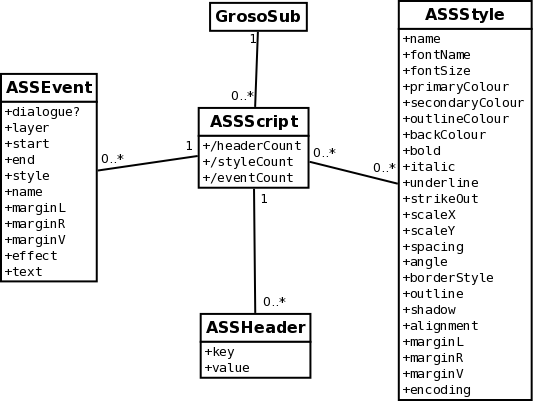
\includegraphics[width=\columnwidth, natwidth=555pt, natheight=402pt]{Pictures/Chapter4/Analisia/DE.png}
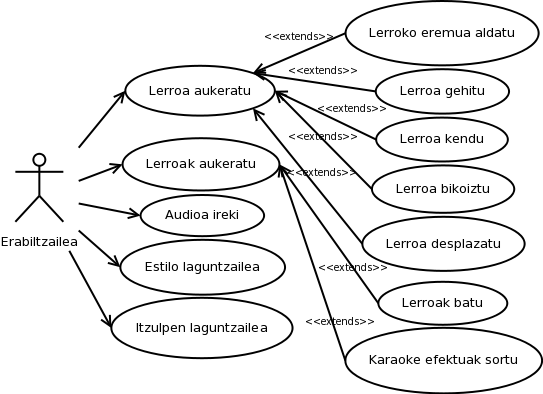
\includegraphics[scale=0.4]{Pictures/Chapter4/Analisia/EKE-Script.png}
\caption{EKE - Script-a irekita egoera}
\label{eke-script}
\end{center}
\end{figure}
\noindent\\
\textbf{ID:} S01.\\
\textbf{Erabilpen kasua:} Lerroak aukeratu.\\
\textbf{Aktoreak:} Erabiltzailea.\\
\textbf{Deskribapena:} Script-ean dagoen lerro bat edo gehiago aukeratzen ditu ondoren bere gainean zenbait eragiketa egiteko.\\
\textbf{Aurrebaldintzak:}  Script-a kargatuta dago eta gutxienez lerro bat dauka.\\
\textbf{Postbaldintzak:} Lerroak aukeratuta geratzen dira.\\
\textbf{Gertaera fluxu normala:}
\begin{enumerate}
	\item \textit{Erabiltzailea:} Script-ean dagoen lerro bat edo gehiago aukeratuko ditu.
	\item \textit{Sistema:} Erabiltzaileak aukeratutako lerroak markatuko ditu interfazean.
	\item \textit{Sistema:} Lerro bakarra aukeratu bada, honen datuak kargatuko ditu interfazean.
\end{enumerate}
\line(1,0){390}\\
\noindent\\
\textbf{ID:} S02.\\
\textbf{Erabilpen kasua:} Lerroko eremua aldatu.\\
\textbf{Aktoreak:} Erabiltzailea.\\
\textbf{Deskribapena:} Aukeratutako lerroko eremu baten edukia aldatzen du.\\
\textbf{Aurrebaldintzak:} Lerro bat aukeratuta dago.\\
\textbf{Postbaldintzak:} Aldatutako eremua lerroan gordeta geratuko da.\\
\textbf{Gertaera fluxu normala:}
\begin{enumerate}
	\item \textit{Sistema:} Aukeratutak lerroaren eremu guztiak eta hauen balioak erakutsiko ditu.
	\item \textit{Erabiltzailea:} Eremu bat aukeratuko du eta honen balioa aldatuko du.
	\item \textit{Erabiltzailea:} Beste eremu bat aldatzeko (2. urratsera) edo aldaketak gordetzeko agindua emango du.
	\item \textit{Sistema:} Lerroan egindako aldaketak gordeko dira.
\end{enumerate}
\line(1,0){390}\\
\noindent\\
\textbf{ID:} S03.\\
\textbf{Erabilpen kasua:} Lerroa gehitu.\\
\textbf{Aktoreak:} Erabiltzailea.\\
\textbf{Deskribapena:} Lerro berri bat gehituko du script-ean.\\
\textbf{Aurrebaldintzak:} Lerro bat aukeratuta dago.\\
\textbf{Postbaldintzak:} Lerro berria script-ean gehituko da.\\
\textbf{Gertaera fluxu normala:}
\begin{enumerate}
	\item \textit{Erabiltzailea:} Aukeratutako lerroaren aurrean edo atzean sartzeko aukeratuko du.
	\item \textit{Sistema:} Erabiltzaileak aukeratutako lekuan txertatuko du lerro berria defektuzko informazioarekin.
\end{enumerate}
\textbf{Gertaera fluxu alternatiboa:}
\begin{itemize}
	\item 0. urratsa: ez badago lerrorik aukeratuta script-ean:
		\begin{enumerate}
		\item \textit{Sistema:} Lerro berri bat gehituko du.
		\end{enumerate}
\end{itemize}
\line(1,0){390}\\
\noindent\\
\textbf{ID:} S04.\\
\textbf{Erabilpen kasua:} Lerroa kendu.\\
\textbf{Aktoreak:} Erabiltzailea.\\
\textbf{Deskribapena:} Aukeratutako lerroa script-etik ezabatzen du.\\
\textbf{Aurrebaldintzak:} Lerro bat aukeratuta dago.\\
\textbf{Postbaldintzak:} Lerroa script-etik ezabatuko da.\\
\textbf{Gertaera fluxu normala:}
\begin{enumerate}
	\item \textit{Sistema:} Erabiltzaileak aukeratutako lerroa ezabatuko du script-etik
\end{enumerate}
\line(1,0){390}\\
\noindent\\
\textbf{ID:} S05.\\
\textbf{Erabilpen kasua:} Lerroa bikoiztu.\\
\textbf{Aktoreak:} Erabitzailea.\\
\textbf{Deskribapena:} Aukeratutako lerroaren kopia bat egingo du aukeratutako lerroaren azpian.\\
\textbf{Aurrebaldintzak:} Lerro bat aukeratuta dago.\\
\textbf{Postbaldintzak:} Aukeratutako lerroa bikoiztuta geratuko da.\\
\textbf{Gertaera fluxu normala:}
\begin{enumerate}
	\item \textit{Sistema:} Lerro berri bat sortuko du aukeratutakoaren azpian eta bertan aukeratutako lerroaren datuak sartuko ditu.
\end{enumerate}
\line(1,0){390}\\
\noindent\\
\textbf{ID:} S06.\\
\textbf{Erabilpen kasua:} Lerroak desplazatu.\\
\textbf{Aktoreak:} Erabiltzailea.\\
\textbf{Deskribapena:} Aukeratutako lerroen denborak desplazatzen ditu.\\
\textbf{Aurrebaldintzak:} Gutxienez lerro bat aukeratuta dago.\\
\textbf{Postbaldintzak:} Aukeratutako lerroen denborak desplazatuta geratzen dira.\\
\textbf{Gertaera fluxu normala:}
\begin{enumerate}
	\item \textit{Sistema:} Lerroak desplazatzeko aukerak erakutsiko ditu interfazean.
	\item \textit{Erabiltzailea:} Desplazatu nahi dituen denborak (hasiera denbora, bukaera denbora edo biak) eta zenbat desplazatu nahi dituen aukeratuko du.
	\item \textit{Sistema:} Aukeratutako lerroen denborak aldatuko ditu erabiltzaileak emandako datuekin.
\end{enumerate}
%\line(1,0){390}\\
\noindent\\
\textbf{ID:} S07.\\
\textbf{Erabilpen kasua:} Lerroak batu.\\
\textbf{Aktoreak:} Erabiltzailea.\\
\textbf{Deskribapena:} Aukeratuta dauden lerroak kateatzen ditu.\\
\textbf{Aurrebaldintzak:} 2 lerro gutxienez aukeratuta daude.\\
\textbf{Postbaldintzak:} Aukeratako lerroak kateatuta dituen lerro berri bat sortzen da.\\
\textbf{Gertaera fluxu normala:}
\begin{enumerate}
	\item \textit{Sistema:} Lerro berri bat sortzen du.
	\item \textit{Sistema:} Aukeratutako lerroen edukia (testua) kateatzen du eta denborak egokitzen ditu (hasiera denboren minimoa eta bukaera denboren maximoa).
	\item \textit{Sistema:} Aukeratutako lerroak ezabatzen ditu.
\end{enumerate}
\line(1,0){390}\\
\noindent\\
\textbf{ID:} S08.\\
\textbf{Erabilpen kasua:} Estilo laguntzailea.\\
\textbf{Aktoreak:} Erabiltzailea.\\
\textbf{Deskribapena:} Estilo laguntzailea kargatuko du.\\
\textbf{Aurrebaldintzak:} Script-a kargatuta dago.\\
\textbf{Postbaldintzak:} Estilo laguntzailea kargatuko du.\\
\textbf{Gertaera fluxu normala:}
\begin{enumerate}
	\item \textit{Sistema:} Script-ean dauden estiloak eta uneko lerroaren testua eta aktorea erakutsiko ditu interfazean.
	\item \textit{Erabiltzailea:} Xagua edo teklatuaren bidez estilo bat aukeratuko du.
	\item \textit{Sistema:} Uneko lerroari aukeratutako estiloa ezarriko dio eta hurrengo lerroa kargatuko du interfazean.
\end{enumerate}
\line(1,0){390}\\
\noindent\\
\textbf{ID:} S09.\\
\textbf{Erabilpen kasua:} Itzulpen laguntzailea.\\
\textbf{Aktoreak:} Erabiltzailea.\\
\textbf{Deskribapena:} Itzulpen laguntzailea kargatuko du.\\
\textbf{Aurrebaldintzak:} Script-a kargatuta dago.\\
\textbf{Postbaldintzak:} Itzulpen laguntzailea kargatuko du.\\
\textbf{Gertaera fluxu normala:}
\begin{enumerate}
	\item \textit{Sistema:} Uneko lerroaren testua erakutsiko du interfazean.
	\item \textit{Erabiltzailea:} Lerro horren itzulpena sartuko du.
	\item \textit{Sistema:} Uneko lerroaren testua aldatuko du erabiltzaileak sartu duenarekin eta hurrengo lerroa erakutsiko du interfazean.
\end{enumerate}

\newpage
\section{Diseinua}
\subsection{Dokumentuetan oinarritutako aplikazioak}
Gure aplikazioak oso komunak diren funtzionalitate batzuk izan behar ditu: fitxategiak ireki, berriak sortu, itxi, etab. Aplikazio hauek dokumentuetan oinarritutakoak dira, eta oso komunak direnez, Cocoa API-ak hauek garatzeko erreztasun asko ematen ditu. \textbf{MVC}\footnote{Model View Controller} patroia jarraituko da diseinua egiterako orduan, nahiz eta klase batzuk mota bat baino gehiagokoak izango diren aurrerago ikusiko dugunez.
\subsubsection{Dokumentu arkitektura}
Horrelako aplikazioak gauzatzeko hiru klase eskaintzen ditu Cocoa-k. Lehenik eta behin \texttt{NSDocument} klasea daukagu. Honen azpiklase bat sortuko dugu dokumentuaren (ASS fitxategia gure kasuan) egitura gordetzeko. Nahiz eta zenbait dokumentu formatu onartuko dituen programak (ASS, SRT eta TXT), ASS-rekin lan egingo du barrutik, beraz azpiklase bakarra sortuko dugu. Klase hau \textit{Model} eta \textit{Controller} motakoa izango da.

Ondoren \texttt{NSWindowController} klasea daukagu. Sortuko dugun aplikazioak lehio bakarra edukiko badu, honen azpiklasea egitea ez da beharrezkoa izango. Gure kasuan lehio bat baino gehiago edukiko dugu dokumentu bakar batentzako, beraz lehio mota bakoitzeko azpiklase bat sortuko dugu. Klaseak interfazearen ekintzak jasoko ditu eta \textit{Model} klasea eguneratuko du. Gainera, azpiklase bakoitza \textbf{NIB} fitxategi konkretu batera lotuta egongo da, non interfazea gordeko den (modu grafikoan editatzen dira fitxategi hauek interfaze grafikoa osatzeko). Hau \textit{Controller} motako klasea da.

Azkenik \texttt{NSDocumentController} klasearekin aurkituko gara, baina honen azpiklaserik ez dugu beharko. Honen eginkizuna dokumentuak maneiatzea da: berriak sortzea, ixtea, etab.

\subsubsection{Ohiko atazak}
Lehen esan bezala, badaude programa hauetan oso ohikoak diren funtzionalitate batzuk, eta dokumentu arkitekturak lana asko errazten digu hauek inplementatzeko. \texttt{NSDocument}-en azpiklasean bi metodo inplementatu beharko dira:
\begin{itemize}
\item \texttt{-dataOfType:error:}:

\texttt{NSData} motako objektu bat (\texttt{NSString} bat kodifikazioa espezifiko batekin, \textbf{UTF8} gure kasuan) itzuli behar du dokumentuaren edukiarekin fitxategi batean gordetzeko. \texttt{typeName} parametroarekin jakingo dugu zein den fitxategiaren formatua.

\item \texttt{-readFromData:ofType:error:}:

\texttt{NSData} motako objektu bat eta fitxategiaren formatua jasotzen du. Bere eginkizuna zera da: edukia irakurtzea eta dokumentuko datu egiturak betetzea.
\end{itemize}

Erabilpen kasu hauen sekuentzia diagramak ez dira egingo: G01 - Fitxategia ireki, G02 - Script berria sortu eta G03 - Fitxategia gorde, Apple-en dokumentazioan\footnote{Apple-en dokumentazioko\cite{ap:dba} 29. orrialdean} aurkitu daitezkeelako, nahiz eta apur bat zahartuta egon (goian aipatutako metodoak ez dira erabiltzen, hauen ordez apur bat zaharragoak baina eginkizun berdina dutenak erabiltzen dira).

Sekuentzia diagramak ikusita, guk oso gutxi programatu beharko dugu (bi funtzio) fitxategiak ireki, itxi eta gordetzeko, kode asko aurreztuz (adibidez ez dugu fitxategia aukeratzeko panela maneiatu beharko edo dokumentuaren instantzia berria sortu beharko).

\subsubsection{Desegin/Berregin}
Aukera hauek inplementatzeko dokumentu arkitekturak ere lana asko erreztuko digu. \texttt{NSDocument}-ek \texttt{NSUndoManager} en instantzia bat dauka. Adibidez, aplikazioan lerro berri bat gehitzen dugunean, \texttt{NSUndoManager}-ean kontrako ekintza erregistratuko dugu, kasu honetan lerroa kentzea. Azken finean bi pila dauzka \texttt{NSUndoManager}-ek, bat desegiteko ekintzekin eta beste bat berregiteko ekintzekin. Desegitea aukeratzen dugunean, berregiteko pilan txertatuko da kontrako ekintza eta alderantziz. Menuko aukerak ere automatikoki kudeatuko dira guk ezer egin gabe.

\subsubsection{Dokumentuaren egoera}
Dokumentuan aldaketaren bat egin badugu, dokumentuaren aldaketa kontagailua inkrementatuko dugu. Kontagailu hau 0 ez bada, dokumentua zikin dagoela esango dugu, hau da, fitxategi sisteman dagoen fitxategia eta aplikazioan kargatuta dagoen dokumentua ez dira berdinak. Programa ixten saiatzen bagara, mezu bat agertuko zaigu zer egin nahi dugun galdetuz (gorde, ez gorde edo ezeztatu).

Aldaketaren bat desegiten badugu, kontagailua murriztuko da, eta fitxategia gordetzen badugu, kontagailuaren balioa 0 izango da berriz ere.

Aurreko kasuetan bezala, esfortzu gutxirekin (kode lerrorik gabe), funtzionalitate hau inplementatuta edukiko dugu.

\subsubsection{Informazio gehiago}
Atal honetan ikusi dugunez, erraztasun asko ematen dizkigu dokumentu arkitekturak, baina askoz gauza gehiago egiteko ere gai da. Informazio gehiago aurkitu daiteke Apple-ek eskaintzen duen dokumentazioan\cite{ap:dba}.

\subsection{Notifikazio bidezko komunikazioa}
Geroago sekuentzia diagrametan ikusiko denez, objektuen arteko zenbait komunikazioa notifikazio bidez egin dira. Exekutatzen ari den aplikazio orok \textit{NSNotificationCenter} klasearen instatzia bat du, aplikazioaren edozein partetik atzigarria dena. Bertan notifikazioak \textbf{bidaliko} dira alde batetik, eta notifikazioen zain \textbf{erregistratuko} dira zenbait objektu. Erregistratzeko unea instantzia sortzerakoan da, eta bertan azalduko da zein notifikazioren zain erregistratu, noren notifikazioak jaso, etab. eta instantzia suntsitzean erregistratuta zegoena ezabatu behar da. Notifikazioa iristen direnean metodo konkretu bat exekutatuko du instantzia, metodo horien parametroa bakarra izanda: \textit{NSNotification} motako objektu bat bidaltzailearen informazioarekin.
 
Adibidez interfazean agertzen diren tauletan (\textit{NSTableView} klasekoak) erabiltzen da: erabiltzaileak lerro bat aukeratzen duenean notifikazioa bat bidaltzen da: NSTableViewSelectionDidChangeNotification izenekoa. \textit{ASSScriptController} klasean notifikazio horren zain geratu gara, eta iristen denean lehioaren goiko eremuetan aukeratutako lerroaren informazioa kargatuko da.

Guzti hau beste modu batean inplementatu daiteke, \textbf{delegate} izeneko loturen bidez. Zenbait klaseek \textit{delegate} motako metodoak dituzte, eta hauek exekutatzeko klase horren instantziak lotuta egon behar dira beste klase baten instantziarekin, \textit{delegate} loturaren bidez Interface Builder-etik. Aurreko kasuan adibidez, \textit{NSTableView}-k badu horrelako metodo bat: tableViewSelectionDidChange, lehenago aipatu dugunaren gauza berdina egiten duena. Bien desberdintasuna hau da: Instantzia batek \textit{delegate} bidez beste instantzia batekin eduki dezake bakarrik lotura, eta notifikazio bidez instantzia batek bidali ditzake notifikazioak eta \textit{n} instantziek jaso ahal dute.

Beste gauza baterako erabili dira notifikazioak aplikazioan, adibidez G08 erabilpen kasuan, goiburuko bat ezabatzerakoan \textit{ASSScript} klaseak ezabatzen du dagokion datu egituratik, eta goiburuko editorearen kontrolatzaileak (\textit{ASSHeadersController}) jakin beharko du goiburukoak aldatu direla zerrenda berriro kargatzeko. Momentu honetan pentsa daiteke: "Zergaitik ez egin zuzenean objektuen arteko mezu baten bidez, ASSScript-etik ASSHeadersController-era?", eta erantzuna sinplea da, ASSHeadersController-en instantzia bat ez da beti egongo, goiburukoen kudeaketarako lehioa ixterakoan instantzia suntsituko delako. Horrela, goiburukoak aldatzerakoan (goiburuko kudeatzailetik, edo adibidez Desegin/Berregin aukeretatik) notifikazioa bidaliko da, eta ASSHeadersController-en instantzia bat badago memorian notifikazioa jasotzerakoan zerbait egingo du. Ez badago instantziarik momentu horretan notifikazioa galduko da eta ez da ezer gertatuko.

Mota honetako komunikazioak aurrerago ikusiko ditugun sekuentzia diagrametan modu sinplifikatuan adierazi dira: beste objektuen arteko metodo bat izango balitz bezala, baina geziaren lerroa marra soil bat izan ordez marra eta puntuak tartekatzen dituena erabiliz.

\subsection{Klase diagrama}

\newpage
\subsection{Sekuentzia diagramak}

\subsubsection{G04 - Goiburukoak kudeatu}
\begin{figure}[htp]
\begin{center}
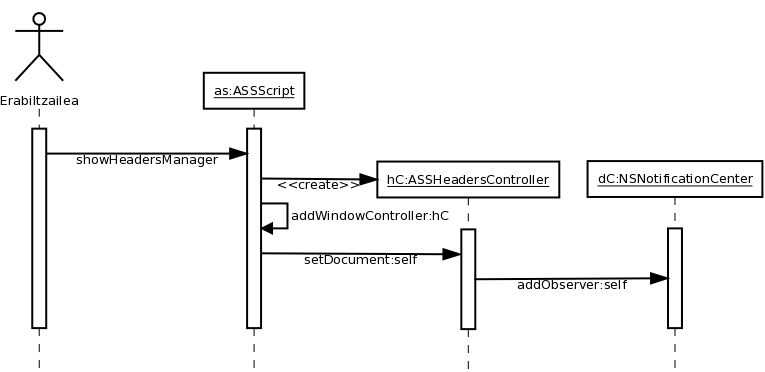
\includegraphics[scale=0.35]{Pictures/Chapter4/Diseinua/G04.png}
\caption{G04 - Goiburukoak kudeatu}
\label{g04d}
\end{center}
\end{figure}

\subsubsection{G05 - Goiburukoa sortu}
\begin{figure}[htp]
\begin{center}
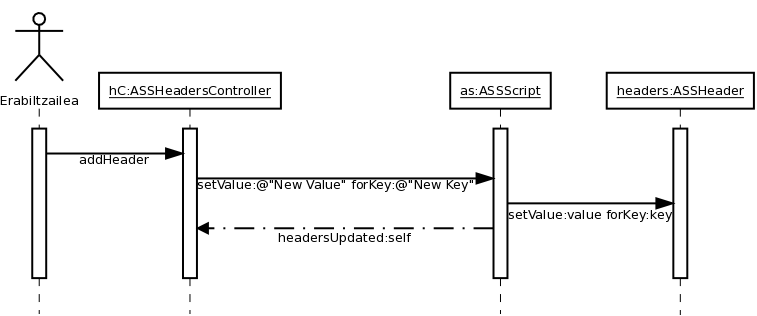
\includegraphics[scale=0.35]{Pictures/Chapter4/Diseinua/G05.png}
\caption{G05 - Goiburukoa sortu}
\label{g05d}
\end{center}
\end{figure}

\newpage
\subsubsection{G06 - Goiburukoa aukeratu}
\begin{figure}[htp]
\begin{center}
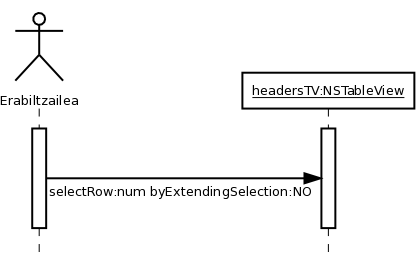
\includegraphics[scale=0.4]{Pictures/Chapter4/Diseinua/G06.png}
\caption{G06 - Goiburukoa aukeratu}
\label{g06d}
\end{center}
\end{figure}


\subsubsection{G07 - Goiburukoa editatu}
\begin{figure}[htp]
\begin{center}
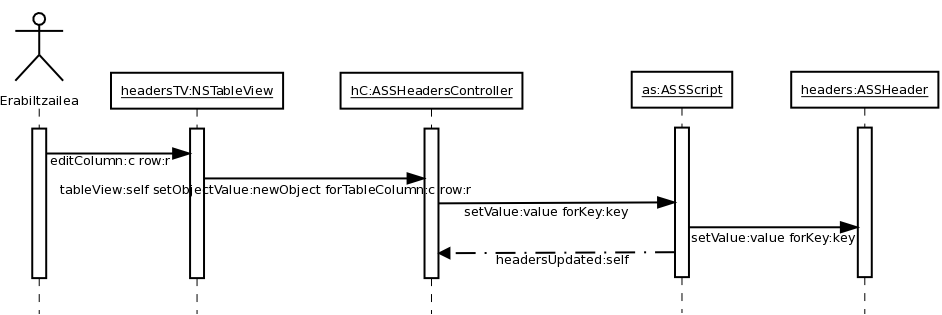
\includegraphics[scale=0.33]{Pictures/Chapter4/Diseinua/G07.png}
\caption{G07 - Goiburukoa editatu}
\label{g07d}
\end{center}
\end{figure}

\newpage
\subsubsection{G08 - Goiburukoa ezabatu}
\begin{figure}[htp]
\begin{center}
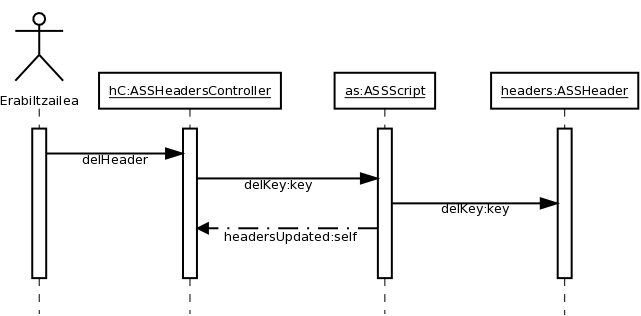
\includegraphics[scale=0.4]{Pictures/Chapter4/Diseinua/G08.png}
\caption{G08 - Goiburukoa ezabatu}
\label{g08d}
\end{center}
\end{figure}


\subsubsection{G09 - Estiloak kudeatu}
\begin{figure}[htp]
\begin{center}
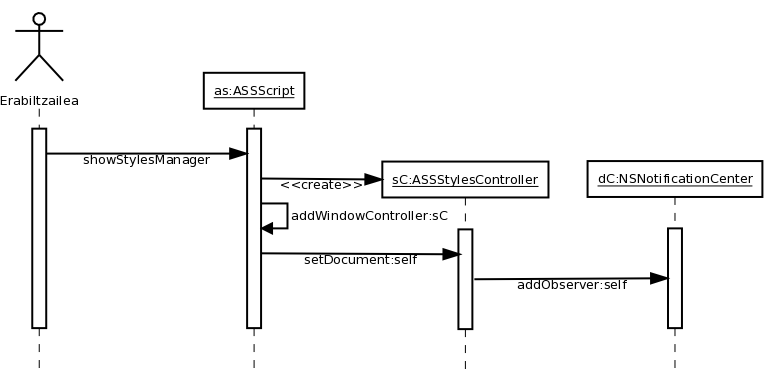
\includegraphics[scale=0.35]{Pictures/Chapter4/Diseinua/G09.png}
\caption{G09 - Estiloak kudeatu}
\label{g09d}
\end{center}
\end{figure}

\newpage
\subsubsection{G10 - Estilo berria sortu}
\begin{figure}[htp]
\begin{center}
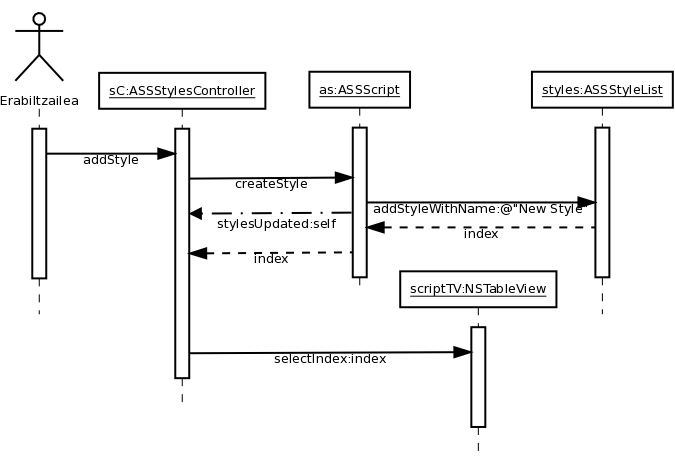
\includegraphics[scale=0.35]{Pictures/Chapter4/Diseinua/G10.png}
\caption{G10 - Estilo berria sortu}
\label{g10d}
\end{center}
\end{figure}


\subsubsection{G11 - Estiloa aukeratu}
\begin{figure}[htp]
\begin{center}
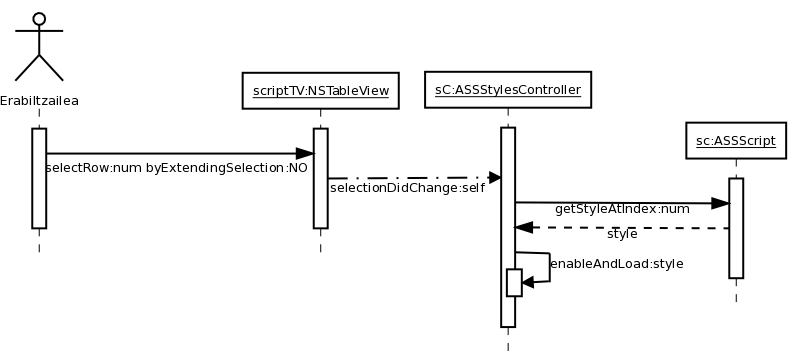
\includegraphics[scale=0.35]{Pictures/Chapter4/Diseinua/G11.png}
\caption{G11 - Estiloa aukeratu}
\label{g11d}
\end{center}
\end{figure}

\newpage
\subsubsection{G12 - Estiloa editatu}
\begin{figure}[htp]
\begin{center}
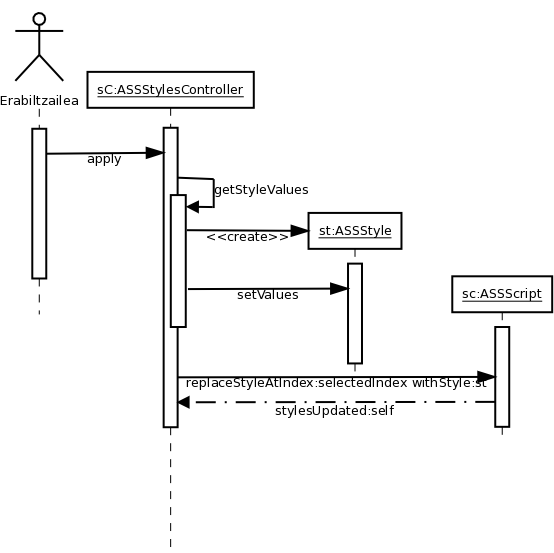
\includegraphics[scale=0.3]{Pictures/Chapter4/Diseinua/G12.png}
\caption{G12 - Estiloa editatu}
\label{g12d}
\end{center}
\end{figure}


\subsubsection{G13 - Estiloa kopiatu}
\begin{figure}[htp]
\begin{center}
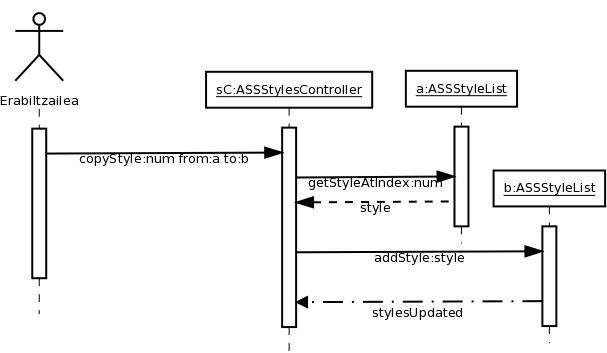
\includegraphics[scale=0.35]{Pictures/Chapter4/Diseinua/G13.png}
\caption{G13 - Estiloa kopiatu}
\label{g13d}
\end{center}
\end{figure}

\newpage
\subsubsection{G14 - Estiloa ezabatu}
\begin{figure}[htp]
\begin{center}
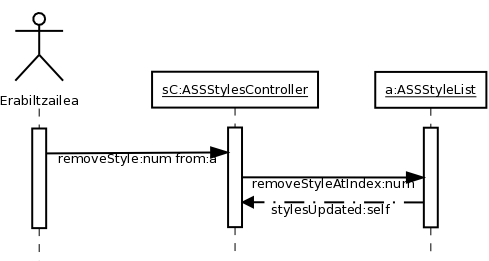
\includegraphics[scale=0.35]{Pictures/Chapter4/Diseinua/G14.png}
\caption{G14 - Estiloa ezabatu}
\label{g14d}
\end{center}
\end{figure}


\subsubsection{S01 - Lerroak aukeratu}
\begin{figure}[htp]
\begin{center}
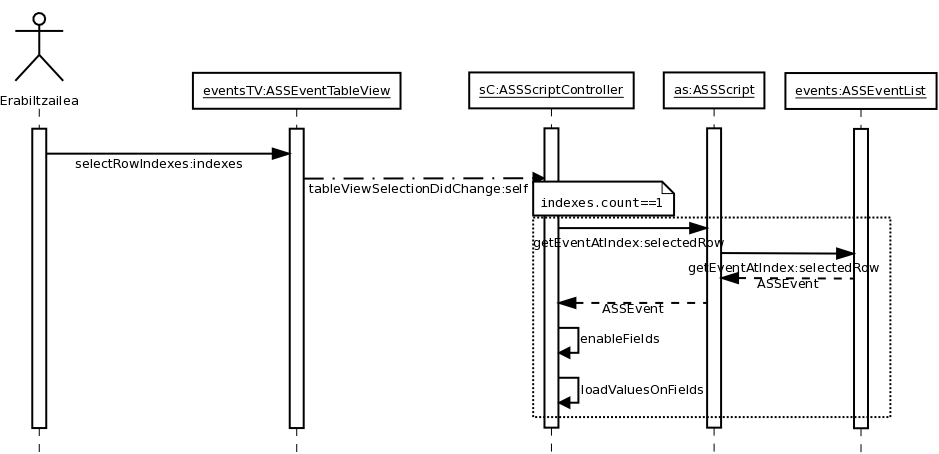
\includegraphics[scale=0.3]{Pictures/Chapter4/Diseinua/S01.png}
\caption{S01 - Lerroak aukeratu}
\label{s01d}
\end{center}
\end{figure}

\newpage
\subsubsection{S02 - Lerroko eremua aldatu}
\begin{figure}[htp]
\begin{center}
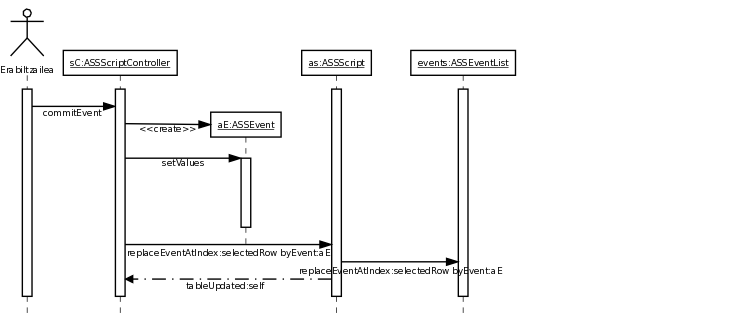
\includegraphics[scale=0.5]{Pictures/Chapter4/Diseinua/S02.png}
\caption{S02 - Lerroko eremua aldatu}
\label{s02d}
\end{center}
\end{figure}


\subsubsection{S03 - Lerroa gehitu}
\begin{figure}[htp]
\begin{center}
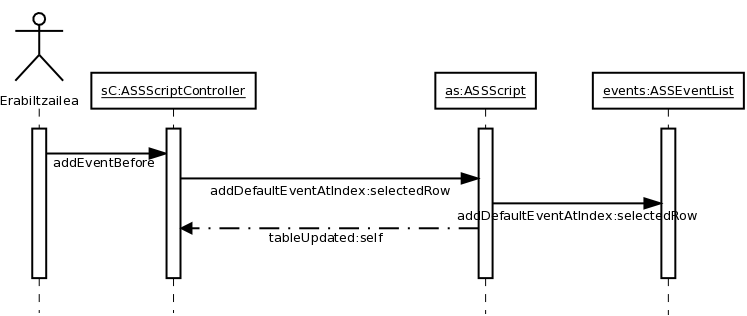
\includegraphics[scale=0.35]{Pictures/Chapter4/Diseinua/S03.png}
\caption{S03 - Lerroa gehitu}
\label{s03d}
\end{center}
\end{figure}

\newpage
\subsubsection{S04 - Lerroa kendu}
\begin{figure}[htp]
\begin{center}
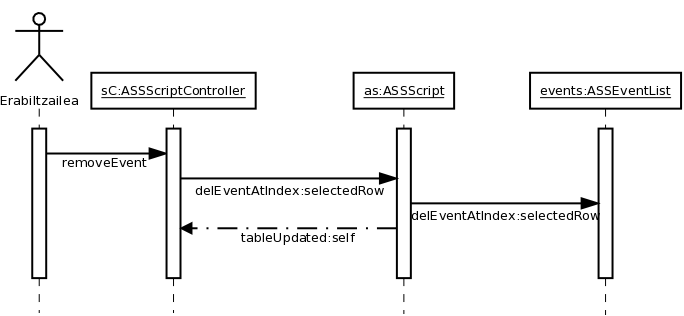
\includegraphics[scale=0.35]{Pictures/Chapter4/Diseinua/S04.png}
\caption{S04 - Lerroa kendu}
\label{s04d}
\end{center}
\end{figure}


\subsubsection{S05 - Lerroa bikoiztu}
\begin{figure}[htp]
\begin{center}
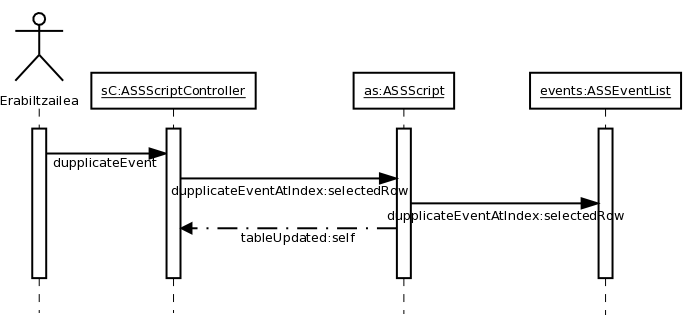
\includegraphics[scale=0.35]{Pictures/Chapter4/Diseinua/S05.png}
\caption{S05 - Lerroa bikoiztu}
\label{s05d}
\end{center}
\end{figure}

\newpage
\subsubsection{S06 - Lerroak desplazatu}
\begin{figure}[htp]
\begin{center}
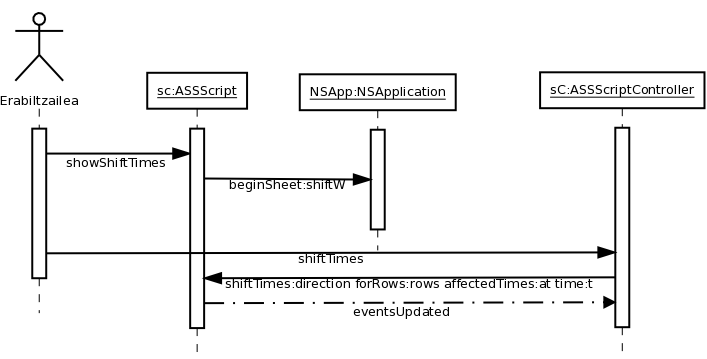
\includegraphics[scale=0.35]{Pictures/Chapter4/Diseinua/S06.png}
\caption{S06 - Lerroak desplazatu}
\label{s06d}
\end{center}
\end{figure}


\subsubsection{S07 - Lerroak batu}
\begin{figure}[htp]
\begin{center}
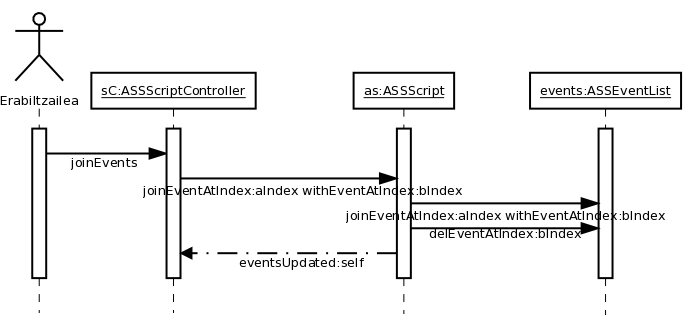
\includegraphics[scale=0.35]{Pictures/Chapter4/Diseinua/S07.png}
\caption{S07 - Lerroak batu}
\label{s07d}
\end{center}
\end{figure}

\newpage
\subsubsection{S08 - Estilo laguntzailea}
\begin{figure}[htp]
\begin{center}
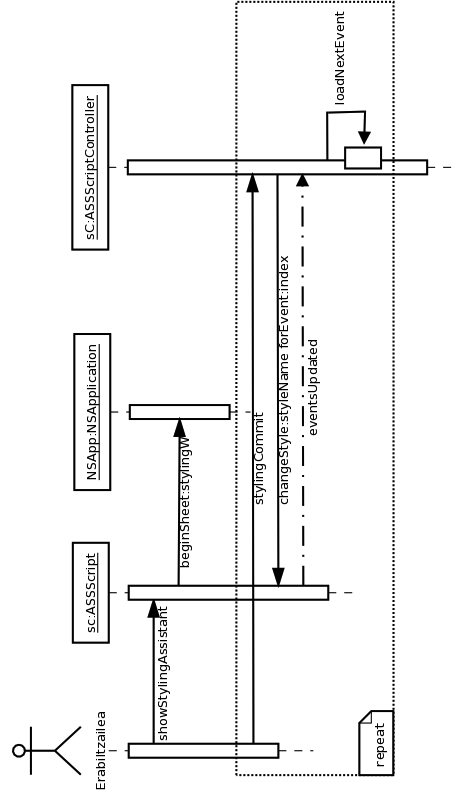
\includegraphics[scale=0.4]{Pictures/Chapter4/Diseinua/S08.png}
\caption{S08 - Estilo laguntzailea}
\label{s08d}
\end{center}
\end{figure}

\newpage
\subsubsection{S09 - Itzulpen laguntzailea}
\begin{figure}[htp]
\begin{center}
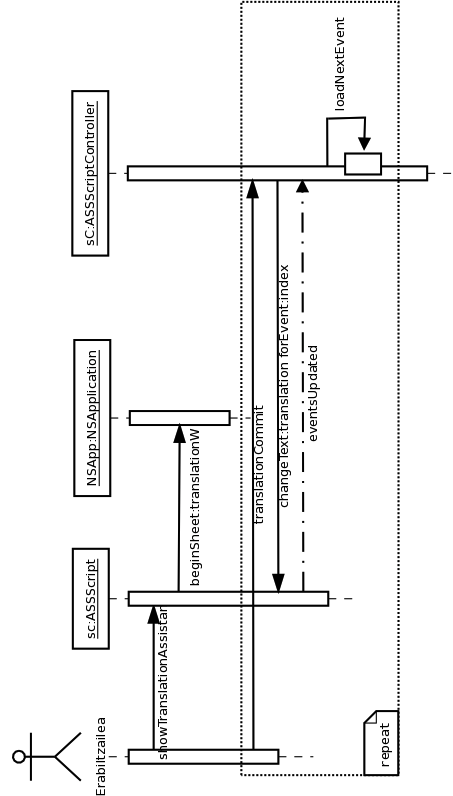
\includegraphics[scale=0.4]{Pictures/Chapter4/Diseinua/S09.png}
\caption{S09 - Itzulpen laguntzailea}
\label{s09d}
\end{center}
\end{figure}


\newpage

\section{Inplementazioa}

\subsection{Kodearen kudeaketa}
Proiektuaren garapenerako bertsioen kontrolerako sistema (RCS\footnote{Revision Control System}) bat erabiltzea ezinbestekoa izan da, garapena ez delako konputagailu bakar batekin egingo, beraz kodea sinkronizatuta edukiko dugu hauetako software bat erabiliz.

SVN\footnote{Subversion} izan da garapenerako aukeratu den RCS-a, batez ere bi arrazoirengandik: ikasleak lehenago erabilia zuelako, horrela ikasketa prozesurik ez egoteko, eta erabili den garapen ingurunean zuzenean erabil daitekeelako.

Lehenago aipatu den moduan, \textit{Assembla.com}-eko zenbait zerbitzu erabili dira proiektuaren bizitzan zehar, eta webgune horrek SVN zerbitzaria eskaintzen duenez hori izan da erabili dena.

SVN-ri esker proiektuko kodea maneiatzea erosoa izan da, zenbait konputagailuetatik lana eginez inongo arazorik izan gabe. Aipatzekoa da ere, memoria hau SVN bidez ere kudeatu dela zerbitzari berdinean, \LaTeX{} fitxategiak azken finean testu fitxategiak direlako.

\subsection{Garapen ingurunea}
Programaren garapenerako eta lehenago aipatu denez, Apple-ek doan eskaintzen duen \textit{Xcode 3 Developer Tools} software konpilazioa erabili da. Bertan tresna asko agertzen dira baina guk ez ditugu guztiak erabili. Kodea idazteko, konpilatzeko, exekutatzeko eta arazteko \textbf{Xcode} erabili da.
\begin{figure}[htp]
\begin{center}
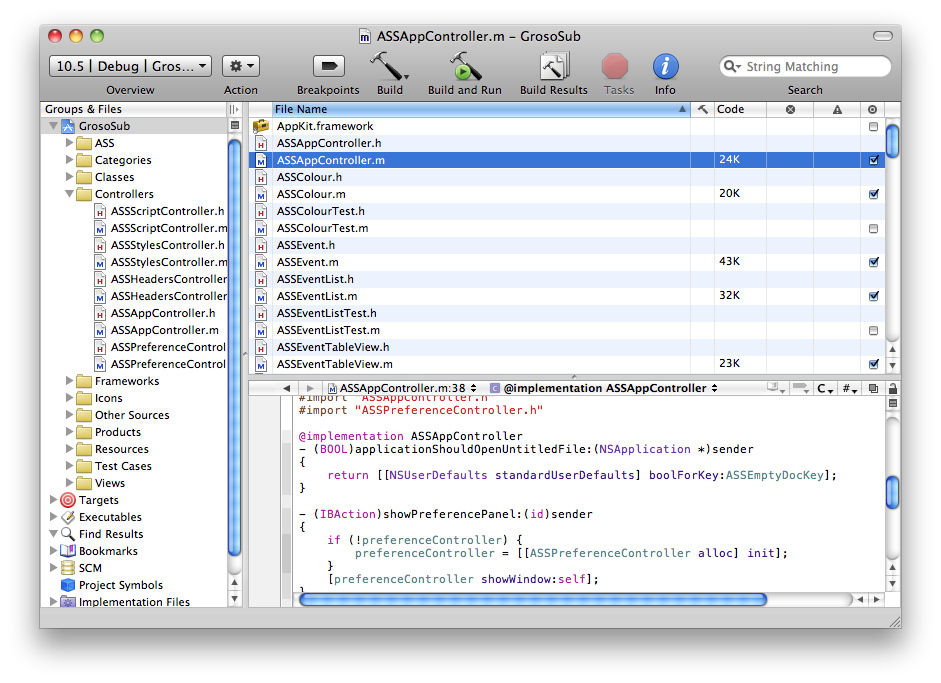
\includegraphics[scale=0.4]{Pictures/Chapter4/Inplementazioa/xcode.png}
\caption{Xcode IDE-a}
\label{xcode}
\end{center}
\end{figure}
\begin{figure}[htp]
\begin{center}
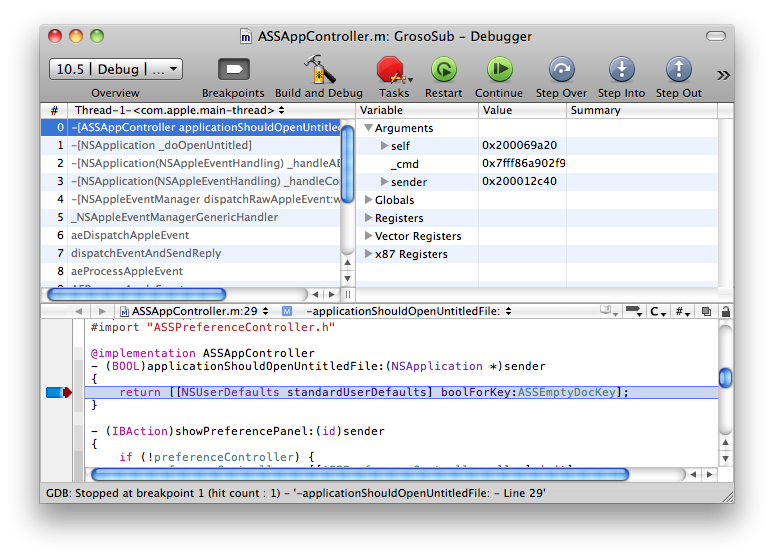
\includegraphics[scale=0.4]{Pictures/Chapter4/Inplementazioa/araztailea.png}
\caption{Xcode IDE-aren araztailea}
\label{debug}
\end{center}
\end{figure}
Barrutik UNIX inguruneetan ohikoak diren tresnak erabiltzen ditu, hala nola \textit{gcc}, \textit{gdb}, etab., baina dena interfaze grafikotik eginda, \ref{xcode} eta \ref{debug}~Irudietan ikusten denez.

Erabili den beste tresna garrantzitsua \textbf{Interface Builder} izan da, izenak esaten duen bezala interfaze grafikoak eraikitzeko tresna. Mac OS X sistemarako garapenean interfazeen sorkuntza desberdinduta dago kodetik. IB-rekin interfaze bat eraikitzerakoan, lehioen barruan elementuak sartuko ditugu: label-ak, testu-kutxak, taulak, etab. Objektuen instantziak ere sar ditzakegu ondoren hauekin loturak egiteko, horrela kodetik atzigarriak izateko interfazearen elementuak eta hauek erakusten duten informazioa.
\begin{figure}[htp]
\begin{center}
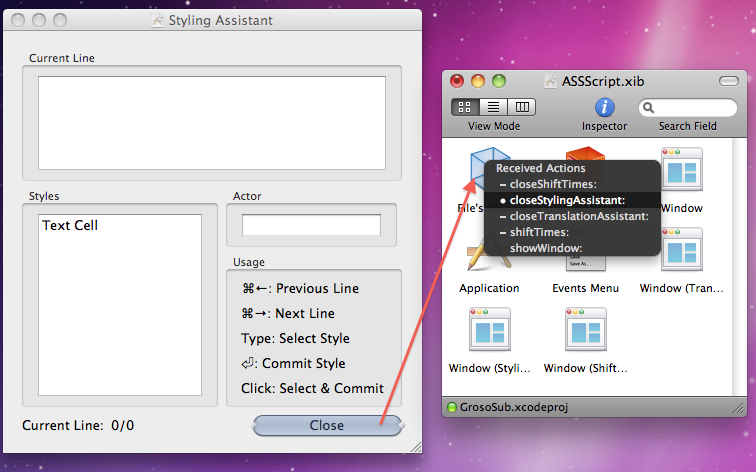
\includegraphics[scale=0.4]{Pictures/Chapter4/Inplementazioa/iblotura.png}
\caption{Interface Builder-en 'Action' motako lotura}
\label{ib1}
\end{center}
\end{figure}
\ref{ib1}~Irudian ikus dezakegu interfazeak edukiko duen lehio bat (ezkerrean), eta botoi batek objektu bati bidaliko dion mezua (lotura). Lotura \textit{File's Owner} ekin egiten da, \textit{NIB} bakoitzak horrelako bat eduki behar du, eta azken finean lehioa kontrolatuko duen klase baten instantzia izango da (kasu honetan \textit{ASSScriptController} klasekoa).

\begin{figure}[htp]
\begin{center}
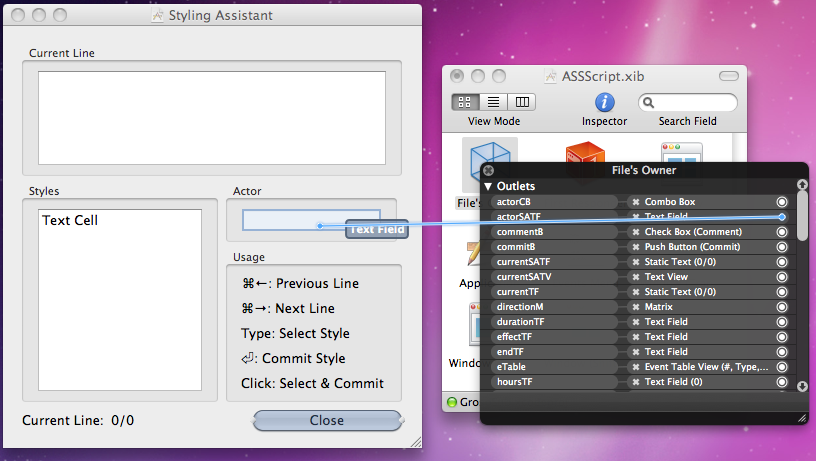
\includegraphics[scale=0.4]{Pictures/Chapter4/Inplementazioa/iblotura2.png}
\caption{Interfaze builder-en 'Outlet' motako lotura}
\label{ib2}
\end{center}
\end{figure}

Aipatu denez, interfazeko datuak atzitu nahiko ditugu kodetik, beraz horrelako loturak ere egin beharko ditugu \ref{ib2}~Irudian ikus dezakeguna hain zuzen ere. Kodean aldagai bat izango dugu \textit{actorSATF} izenekoa irudian ikusten den \textit{textfield}-eko datuak irakurri eta idazteko.

IB-k informazioa \textit{XIB} edo \textit{NIB} formatuko fitxategietan gordetzen du, eta aplikazioa exekutatzerakoan kargatzen da hauen edukia. Gure kasuan zenbait fitxategi desberdin ditugu proiektuan: bat aplikazioaren menu barrarekin, beste bat lehio nagusia eta 'sheet' laguntzaileekin, beste bat estilo editorearen lehioarekin eta azkenik beste bat goiburuko editorearekin. \textit{XIB} eta \textit{NIB} fitxategien funtzioa berdina da baina bereizitasun bakarra dago bien artean, \textit{NIB} fitxategi bitarra da eta \textit{XIB} XML formatuan dago. Azken hau erabili dugu guk SVN-rekin lan egiteko gomendagarriagoak direlako testu fitxategiak.

\subsection{Erabiltzailearen datuak}
Programan exekuzio batetik bestera gorde behar diren datuak dauzkagu, beraz nonbait gorde behar ditugu fitxategietan. Horretarako aplikazioa exekutatzen ari den erabiltzailearen \textit{HOME} katalogoaren barruan gordeko dira datuak, konkretuki \textbf{/Users/erab/Library/} katalogoren barruan.

\subsubsection{Estilo biltegiak}
Kasu honetan, estiloak ASS formatuan bezala gordetzen dira /Users/erab/ Library/Application Support/GrosoSub/styles/ katalogo barruko fitxategi desberdinetan. \textbf{Application Support} katalogoa horretarako erabiltzen dute aplikazio guztiek, mota desberdinetako eta programak maneiatuko dituen datuak gordetzeko. Katalogoa ez bada existitzen programak sortuko du bertan zerbait gordeko duen lehenengo aldian.

\subsubsection{Preferentziak}
Aurrekoarekin alderatuta, preferentzien kontua desberdina da, aplikazio gehienetan ohikoa den funtzio bat denez beste forma batean gorde eta kudeatzen delako. XML formatuko fitxategi batean gordetzen dira preferentziak, /Users/erab/Library/Preferences/com.perryranch.grososub.plist hain zuzen ere. Preferentziak maneiatzeko oso kode gutxi idatzi behar izan da, bakar bakarrik zeintzuk diren preferentzien defektuzko balioak. Erabiltzaileak ezarri dituen balioak hasieran kargatzeko eta programa ixtean gordetzeko Inteface Builder bidez egiten da, \textit{Cocoa bindings} izeneko teknika erabiliz, lehen ikusi dugun modu berdintsuan loturak ezarriz. \ref{prefs}~Irudian ikus daiteke aplikazioaren preferentzia lehioa.
\begin{figure}[htp]
\begin{center}
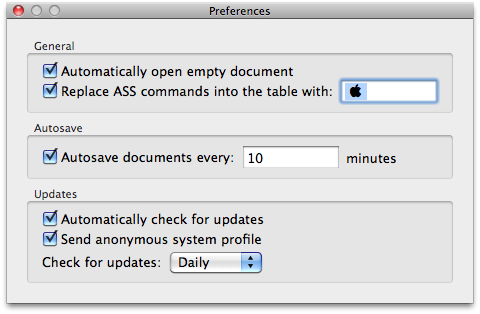
\includegraphics[scale=0.6]{Pictures/Chapter4/Inplementazioa/prefs.png}
\caption{Aplikazioaren preferentzia lehioa}
\label{prefs}
\end{center}
\end{figure}

Erabiltzaileak ezartzen dituen balioak aplikazioaren edozein partetik atzigarriak dira.

\subsection{Eguneraketa automatikoak}
Aplikazioaren eskakizunetan eguneraketa automatikoen kontua aipatzen da, eta horretarako Mac OS sisteman oso erabilia den \textit{framework} bat erabili da: \textbf{Sparkle\footnote{\url{http://sparkle.andymatuschak.org/}}}. Honetarako ere ez dugu kode lerro bakar bat ere idatzi behar izan, beharrezkoa izan den bakarra framework-aren webgunean azaltzen dituzten loturak Interface Builder-en egitea izan da.

Eguneraketen funtzionamendua erraza da: AppCast\footnote{\url{http://connectedflow.com/appcasting/}} formatua jarraitzen duen XML fitxategi bat atzigarri eduki behar dugu internet-en, baita aplikazioaren bertsio desberdinak eta hauen arteko informazioa ere (\textit{ChangeLog}). Horrela konfiguratzen badugu preferentzietan, aplikazioak noizbehinka begiratuko du ea eguneraketarik dagoen, eta horrela bada erabiltzaileari jakinaraziko dio. Honek baiztapena emango du eguneraketa gauzatzeko edo ez, geroagorako utziz edo bertsio konkretu hori ahaztuz.

Bestalde, eta \ref{prefs}~Irudian ikusten den bezala, eguneraketak egiterakoan sistemaren informazioa bidali daiteke (sistemaren bertsioa, hizkuntza, prozesadorea, etab.), garatzaileak ikus dezan zein motako sistemetan exekutatzen den aplikazioa.

Azkenik, erabiltzaileak nahi duenean begiratu dezake ea eguneraketarik dagoen menu-an agertzen den aukera batetik, eta prozesua aipatu dugun berdina izango litzateke.

\subsection{Exekutagarriaren sorkuntza}
Mac OS X sistema eragilea hiru arkitektura desberdinetan erabili daiteke. Alde batetik \textbf{X86} 32 eta 64 biteko makinetan, eta bestetik gero eta gutxiago erabiltzen \textbf{PPC} makinetan, 32 eta 64 bitekoak hauek ere. Sistema eragilearen azkenengo bertsioan (10.6) PPC arkitektura kendu dute, X86 bakarrik geratuz, baina guk gure aplikazioa PPC makinetarako ere eskaini nahi dugu. Horretarako Xcode-ko proiektuan, SDK-ren 10.5 bertsioa aukeratu dugu, eta exekutagarri \textit{Unibertsala} sortzeko esan dugu, hau da, PPC eta X86 arkitekturetarako kode bitarra sortuko dugu aplikazioa konpilatzerakoan. Noski, aplikazioaren tamaina handiago izango da, baina hala ere 3 MiB inguru okupatzen ditu.

Eskakizunetan aipatzen zen aplikazioa instalatzeko erraza izan behar zela, erabiltzaileak konpilatu behar ez izateko. Aplikazioa konpilatzerakoan, .app fitxategi batekin aurkituko gara. Nahiz eta sistemak fitxategi bezala ikusi, benetan katalogo bat da, eta barruan beharrezkoak diren gauza guztiak ditu: exekutagarria (arkitektura desberdinetarako), framework-ak, erabiltzen diren irudiak, ikonoak, itzulpena, etab.

Instalatzeko orduan programa gehienak instalatzen diren moduan egiten da, .app \textit{fitxategi} hori zuzenean \textbf{/Applications/} sistemako katalogora kopiatuz. Sisteman ohikoa den moduan, .app fitxategia \textbf{DMG}\footnote{\url{http://en.wikipedia.org/wiki/Apple_Disk_Image}} baten barruan sartu da. Aplikazioa sistematik ezabatzea ere erraza da, /Applications/ katalogotik ezabatuz nahikoa baita.

\section{Probak}
Softwarearen edozein garapen prozesutan logikoa denez, garatzen dena probatu egin behar da bere funtzionamendua egokia den jakiteko. Aplikazioaren izaera dela eta bi motako probak gauzatu dira.

\subsection{Proba unitarioak}
Aplikazioaren garapenaren hasieran, ASS formatua maneiatzeko beharrezkoa inplementatu zen. Gogoratu beharra dago aplikazioaren formatu 'natiboa' ASS dela, nahiz eta SRT formatuarekin ere lan egin daitekeen, SRT ASS-ren azpimultzo bezala ulertu daitekeelako, beraz aplikazioak barrutik ASS formatuarekin lan egingo du.

Inplementatu ziren klaseak eta hauen metodoak probatzeko proba unitarioak erabili dira, horrela zerbait aldatzean eta probak ondo diseinatuta badaude, probak berriro exekuta daitezke ikusteko ea zerbait apurtu dugun azken aldaketekin.

\subsubsection{SenTestingKit}
Xcode IDE-ak badauka proba unitarioentzako framework bat, SenTestintKit izenekoa. Hasieran Sen:te\footnote{\url{http://www.sente.ch/software/ocunit/}}-k garatu zuen OCUnit izenarekin, baina Xcode 2.1 bertsiotik aurrera Apple-ek eskaintzen duen software konpilazioaren barruan dago izen berriarekin.

Probatu nahi izan dugun klase bakoitzeko beste klase bat sortu dugu, \textit{SenTestCase} klasearen azpliklase direnak. Bertan egin nahi dugun test unitario bakoitzeko metodo bat jarri dugu, horien barruan probatu nahi duguna exekutatuz eta horren emaitza espero genuenarekin konparatuz, SenTestintKit-ek eskaintzen dituen \textbf{Assert} motako funtzioak erabiliz. Hona hemen test baten adibidea:

\begin{verbatimtab}[8]
- (void) testCompare
{
	ASSTime *t1 = [[ASSTime alloc]
			initWithString:@"1:44:03.88"];
	ASSTime *t2 = [[ASSTime alloc]
			initWithString:@"1:44:03.88"];
	ASSTime *t3 = [[ASSTime alloc]
			initWithString:@"1:44:06.88"];
	
	STAssertTrue([t1 compare:t2] == NSOrderedSame,
			@"This should be the same");
	STAssertTrue([t1 compare:t3] == NSOrderedAscending,
			@"t1 should be less than t3");
	STAssertTrue([t3 compare:t2] == NSOrderedDescending,
			@"t3 should be greater than t2");
}
\end{verbatimtab}

ASSTime klasearen hiru instantzia definitzen dira (t1, t2 eta t3), eta ondoren hiru gauza probatzen dira: t1 == t2, t1 $>$ t3 eta t3 $<$ t2. Test horietako bat ez bada betetzen, kodean jarri dugun mezua agertuko da interfazean eta errore bezala markatuko ditu lerroak, jakiteko zein izan den gaizki funtzionatzen duena.

\ref{ocunit}~Irudian ikus daiteke diseinatu diren proba unitario guztiak pasatzen direla arazorik gabe.
\begin{figure}[htp]
\begin{center}
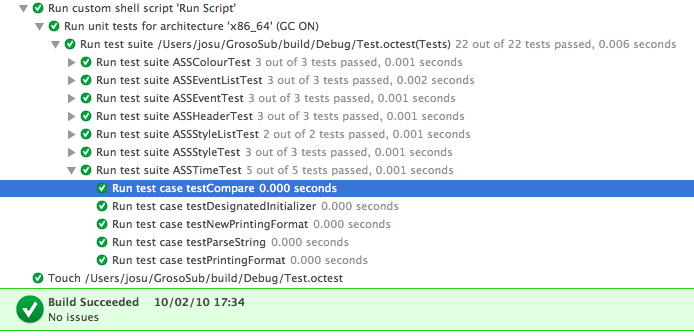
\includegraphics[scale=0.6]{Pictures/Chapter4/Probak/ocunit.png}
\caption{Proba unitarioen exekuzioa}
\label{ocunit}
\end{center}
\end{figure}

Oraingo honetan ere, Apple-ek eskaintzen duen dokumentazioan\cite{ap:ocu} honi buruzko informazio mordoa aurkituko dugu.

\subsubsection{Egin diren probak}
\ref{ocunit}~Irudian ikus dezakegunez 22 proba unitario egin dira guztira honako klaseen funtzionamendu egokia bermatzeko:
\begin{itemize}
	\item ASSColour: \begin{itemize}
		\item Defektuzko balioa espero zena.
		\item Balio maximoa onartzen du.
		\item Ausazko balioa ondo jaso eta itzuli.
	\end{itemize}
	\item ASSEventList: \begin{itemize}
		\item Lista sortzerakoan item bakarra listan.
		\item Txertaketa, ezabaketa eta aldaketen eraginak zuzenak.
		\item Karaktere kate batetik datuak ondo jasotzen dira.
	\end{itemize}
	\item ASSEvent: \begin{itemize}
		\item Defektuzko balioa espero zena.
		\item Karaktere kate batetik datuak ondo jasotzen dira.
		\item Bi ASSEvent-en arteko 'join'-a ondo egiten da.
	\end{itemize}
	\item ASSHeader: \begin{itemize}
		\item Defektuzko balioa espero zena.
		\item Karaktere kate batetik datuak ondo jasotzen dira.
		\item Txertaketa, ezabaketa eta aldaketen eraginak zuzenak.
	\end{itemize}
	\item ASSStyleList: \begin{itemize}
		\item Lista sortzerakoan item bakarra listan.
		\item Karaktere kate batetik datuak ondo jasotzen dira.
	\end{itemize}
	\item ASSStyle: \begin{itemize}
		\item Defektuzko balioa espero zena.
		\item Ausazko ASSStyle bat jaso eta itzuli.
		\item Estiloetan agertzen diren balio boolearrak ondo errepresentatuta irteeran. 
	\end{itemize}
	\item ASSTime: \begin{itemize}
		\item Defektuzko balioa espero zena.
		\item Irteerako karaktere katea ondo sortzen du.
		\item Karaktere kate batetik datuak ondo jasotzen dira.
		\item Karaktere kate batekin zuzenean hasieratu daiteke.
	\end{itemize}
\end{itemize}

\subsection{Proba ez unitarioak}
Nahiz eta proba unitarioak oso ondo egon garapenean zehar behin eta berriz exekutatu ahal ditugulako programaren portaera zuzena dela ikusteko, ezin dira programa osoa probatzeko erabili, adibidez, nola probatu interfaze grafikoa proba unitarioen bidez? SenTestingKit-ek behintzat ez du horrelakorik eskaintzen.

Beraz, aplikazioaren funtzionamendua egiaztatzeko modu bakarra aplikazioa erabiltzea da gauzak ondo dabiltzan edo ez ikusiz. Lana ez da makala, egoera eta ekintza konbinaketa handia delako eta seguraski arazoren bat ez dugu aurkituko. Dena den, proba prozesu hau erraztearren proiektuaren kanpoko zenbait pertsonen laguntza egon da, garapenean zehar aplikazioa erabili izan dutenak eta erroreak aurkitzerakoan komunikatu dituztenak.

Arazo \textit{arraroak} aurkitu direnean Xcode-k eskaintzen duen araztailea erabili da, programaren funtzionamendua pausoz pauso aztertuz errorea aurkitu arte.

\section{Kudeaketa}

\subsection{Jarraipen bilerak}

\subsection{Egoera txostenak}

\subsection{Proiektuan zehar egon diren arazo eta atzerapenak}

\subsection{Amaierako ondorioak}

\subsubsection{Benetako esfortzua}

\subsubsection{Hasierako plangintza vs. amaierako plangintza}
